\section{Introduzione}
\subsection*{Fasi del progetto}
\begin{center}
    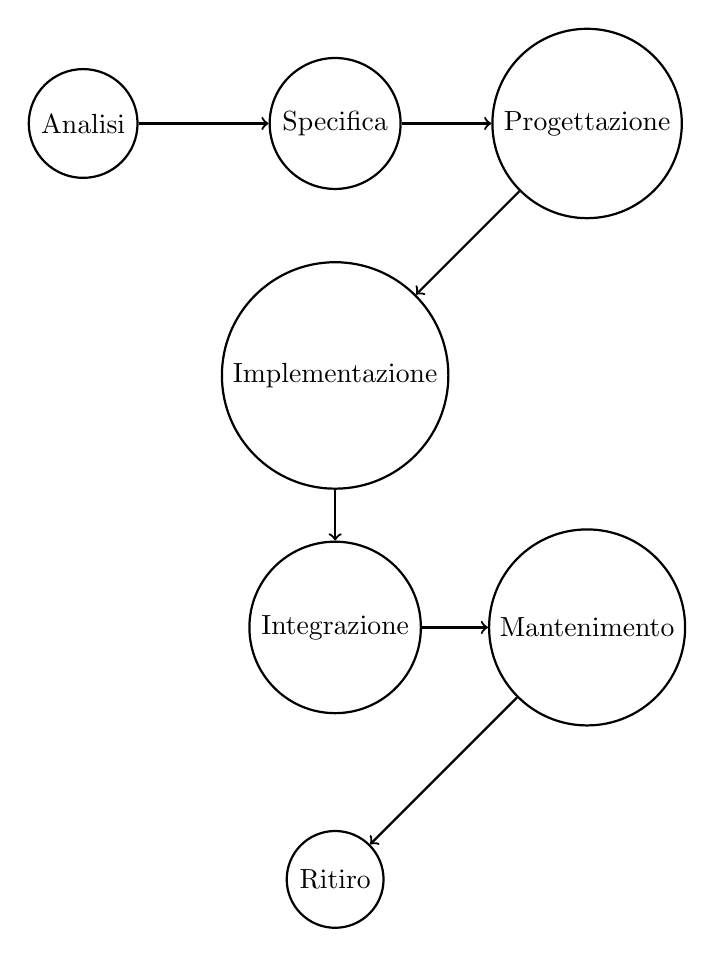
\begin{tikzpicture}[node distance={32mm}, thick, main/.style = {draw, circle}]
        \node[main] (1) {Analisi};
        \node[main] (2) [right of=1] {Specifica};
        \node[main] (3) [right of=2] {Progettazione}; 
        \node[main] (4) [below of=2] {Implementazione};
        \node[main] (5) [below of=4] {Integrazione}; 
        \node[main] (6) [right of=5] {Mantenimento};
        \node[main] (7) [below of=5] {Ritiro};
        \draw[->] (1) -- (2);
        \draw[->] (2) -- (3);
        \draw[->] (3) -- (4);
        \draw[->] (4) -- (5);
        \draw[->] (5) -- (6);
        \draw[->] (6) -- (7);
    \end{tikzpicture}
\end{center}
\subsection*{Specificità del Software}
    \begin{enumerate}
        \item \textbf{\textcolor{cyan}{Fault toulerance}}: capacità del software di essere tollerante ai guasti.
        \item \textbf{\textcolor{cyan}{Difetto latente}}: difetto nascosto che si trova difficilmente in fase di testing; e anche nel caso comparisse è quasi impossibile da ritrovare.
        \item \textbf{\textcolor{cyan}{Robustezza}}: capacità di funzionare anche con input non previsti e/o non testati.
        \item Il software non presenta \textcolor{cyan}{costi materiali} e nemmeno \textcolor{cyan}{costi marginali}, ovvero il costo di un'unità del prodotto.
        \item Infine il software non si consuma nel tempo, ma potrebbe diventare \textcolor{cyan}{obsoleto}.
    \end{enumerate}
\subsection*{La Manutenzione}
    \paragraph{Costi} 
    La fase di manutenzione è quella che richiede costi più alti. 
    Per evitare uno spreco durante questa fase è necessario studiare bene l'analisi dei requisiti, in quanto un errore in questa fase
    si propagherà in modo esponenziale, in termini di costi, nelle fasi successive.
    \break
    \break
    La manutenzione si divide in:
    \begin{itemize}
        \item \textbf{\textcolor{cyan}{Manutenzione Correttiva}}: rimuove gli errori, lasciando invariata la specifica.
        \item \textbf{\textcolor{cyan}{Manutenzione Migliorativa}}: consiste nel cambiare quella che è la specifica, e a sua volta può dividersi in:
            \begin{itemize}
                \item \textcolor{cyan}{Perfettiva}: modifiche per migliorare e/o introdurre nuove funzionalità.
                \item \textcolor{cyan}{Adattiva}: modifiche indotta da cambiamenti esterni, come leggi o modifiche all'hardware o al sistema operativo.
            \end{itemize}
    \end{itemize}
    \subsection*{Stakeholders}
        \begin{itemize}
            \item \textcolor{cyan}{Fornitore}: colui che sviluppa il software.
            \item \textcolor{cyan}{Committente}: chi lo richiede e paga.
            \item \textcolor{cyan}{Utente}: chi lo usa.
        \end{itemize}